\part{Language}
\label{part:lang}

\chapter{Overview of CIVL-C}

\section{Main Concepts}

CIVL-C is an extension of a subset of the C11 dialect of C. It
includes the most commonly-used elements of C, including most of the
syntax, types, expressions, and statements. Missing are some of the
more esoteric type qualifiers, bitwise operations (at least for now),
and much of the standard library.  Moreover, none of the C11 language
elements dealing with concurrency are included, as CIVL-C has its own
concurrency primitives.

The keywords in CIVL-C not already in C begin with the symbol \cckey.
This makes them readily identifiable and also prevents any naming
conflicts with identifiers in C programs.  This means that most legal
C programs will also be legal CIVL-C programs.

One of the most important features of CIVL-C not found in standard C
is the ability to define functions in any scope. (Standard C allows
function definitions only in the file scope.)  This feature is also
found in GNU C, the GNU extension of C.

Another central CIVL-C feature is the ability to \emph{spawn}
functions, i.e., run the function in a new \emph{process} (thread).

\emph{Scopes} and \emph{processes} are the two central themes of
CIVL-C.  Each has a static and a dynamic aspect.  The static scopes
correspond to the lexical scopes in the program---typically, regions
delimited by curly braces \lb \ldots \rb.  At runtime, these scopes
are \emph{instantiated} when control in a process reaches the
beginning of the scope.  Processes are created dynamically by
\emph{spawning} functions; hence the functions are the static
representation of processes.

\section{Example Illustrating Scopes and Processes}

To understand the static and dynamic nature of scopes and processes,
and the relations between them, we consider the (artificial) example
code of Figure \ref{fig:scopecodeex}.  The static scopes in the scope
are numbered from $0$ to $6$.

\begin{figure}[t]
  \centering
  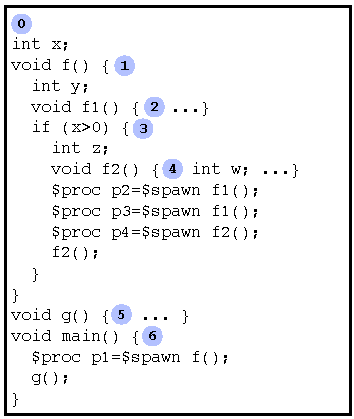
\includegraphics[scale=1.2]{scopeCodeExample}
  \caption{CIVL-C code skeleton to illustrate scope hierarchy}
  \label{fig:scopecodeex}
\end{figure}

\begin{figure}
  \centering
  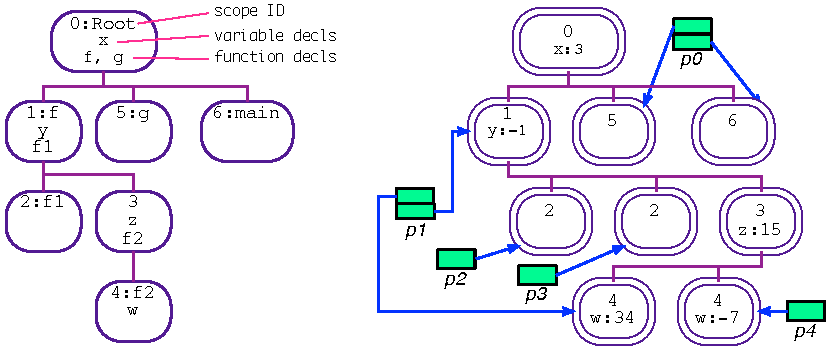
\includegraphics[scale=1.2]{scopeStateExample}
  \caption{Static scope tree and a state for example program}
  \label{fig:scopestateex}
\end{figure}

The static scopes have a tree structure: one scope is a child of
another if the first is immediately contained in the second.  Scope 0,
which is the file scope (or \emph{root} scope) is the root of this
tree.  The static scope tree is depicted in Figure
\ref{fig:scopestateex} (left).  Each scope is identified by its
integer ID.  Additionally, if the scope happens to be the scope of a
function definition, the name of the function is included in this
identifier.  A node in this tree also shows the variables and
functions declared in the scope.  For brevity, we omit the \emph{proc}
variables.

We now look at what happens when this program executes.  Figure
\ref{fig:scopestateex} (right) illustrates a possible state of the
program at one point in an execution.  We now explain how
this state is arrived at.

First, there is an implicit \emph{root function} placed around the
entire code.  The body of the \emph{main} function becomes the body
of the root function, and the \emph{main} function itself disappears.
This minor transformation does not change the structure of the scope
tree.

Execution begins by spawning a process $p_0$ to execute the root
function.  This causes scope $0$ to be instantiated.  An instance of a
static scope is known as a \emph{dynamic scope}, or \emph{dyscopes}
for short.  The dynamic scopes are represented by the ovals with
double borders on the right side of Figure \ref{fig:scopestateex}.
Each dyscope specifies a value for every variable declared in the
corresponding static scope.  In this case, the value $3$ has been
assigned to variable \texttt{x}.

The state of process $p_0$ is represented by a \emph{call stack}
(green).  The entries on this stack are \emph{activation frames}.
Each frame contains two data: a reference to a dyscope (indicated by
blue arrows) and a current location (or programmer counter vaule) in
the static scope corresponding to that dyscope (not shown).  The
dyscope defines the environment in which the process evaluates
expressions and executes statements.  The currently executing function
of a process, corresponding to the top frame in the call stack, can
``see'' only the variables in its dyscope and those of all the
ancestors of its dyscope in the dyscope tree.

Returning to the example, $p_0$ enters scope 6, instanitating that
scope, and then spawns procedure \texttt{f}.  This creates process
$p_1$, with a new stack with a frame pointing to a dyscope
corresponding to static scope 1.  The new process proceed to run
concurrently with $p_0$.  Meanwhile, $p_0$ calls procedure \texttt{g},
which pushes a new entry onto its call stack, and instantiates scope
5.  Hence $p_0$ has two entries on its stack: the bottom one pointing
to the instance of scope 6, the top one pointing to the instance of
scope 5.

Meanwhile, assume $\texttt{x}>0$, so that $p_1$ takes the \emph{true}
branch of the \texttt{if} statement, instantiating scope 3 under the
instance of scope 1.  It then spawns two copies of procedure
\texttt{f1}, creating processes $p_2$ and $p_3$ and two instances of
scope 2.  Then $p_1$ spawns \texttt{f2}, creating process $p_4$ and an
instance of scope 4.  Note that the instance of scope 4 is a child of
the instance of scope 3, since the (static) scope 4 is a child of
scope 3.  Finally, $p_1$ calls \texttt{f2}, pushing a new entry on its
stack and creating another instance of scope 4.  The final state
arrived at is the one shown.

There are few key points to understand:
\begin{itemize}
\item In any state, there is a mapping from the dyscope tree to the
  static scope tree which maps a dyscope to the static scope of which
  it is an instance.  This mapping is a \emph{tree homomorphism},
  i.e., if dyscope $u$ is a child of dyscope $v$, then the static
  scope corresponding to $u$ is a child of the static scope
  corresponding to $v$.
\item A static scope may have any number of instances, including 0.
\item Dynamic scopes are created when control enters the corresponding
  static scope; they disappear from the state when they become
  unreachable.  A dyscope $v$ is ``reachable'' if some process has a
  frame pointing to a dyscope $u$ and there is a path from $u$ up to
  $v$ that follows the parent edges in the dyscope tree.
\item Processes are created when functions are spawned; they disappear
  from the state when their stack becomes empty (either because the
  process terminates normally or invokes the \emph{exit} system
  function).
\end{itemize}

\section{Structure of a CIVL-C program}

A CIVL-C program is structured very much like a standard C program.
In particular, a CIVL-C program may use the preprocessor directives
specified in the C Standard, and with the same meaning.  A source
program is preprocessed, then parsed, resulting in a translation unit,
just as with standard C.  The main differences are the nesting of
function definitions and the new primitives beginning with
\texttt{\$}, which are described in detail in the remainder of this
part of the manual.

A CIVL-C program must begin with the line
\begin{verbatim}
#include <civlc.h>
\end{verbatim}
which includes the main CIVL-C header file, which declares all the
types and other CIVL primitives.

As usual, a translation unit consists of a sequence of variable
declarations, function prototypes, and function definitions in file
scope.  In addition, \emph{assume} statements may occur in the file
scope.  These are used to state assumptions on the input values
to a program.

\chapter{Sequential Elements}

In this chapter we describe the main sequential elements of the
language.  For the most part these are the same as in C.
Primitives dealing with concurrency are introduced in Chapter
\ref{chap:concurrency}.

\section{Types}

\subsection{Standard types inherited from C}

The boolean type is denoted \verb!_Bool!, as in C. Its values are $0$
and $1$, which are also denoted by $\cfalse$ and $\ctrue$,
respectively.

There is one integer type, corresponding to the mathematical integers.
Currently, all of the C integer types \texttt{int}, \texttt{long},
\texttt{unsigned\ int}, \texttt{short}, etc., are mapped to the CIVL
integer type.

There is one real type, corresponding to the mathematical real
numbers. Currently, all of the C real types \texttt{double},
\texttt{float}, etc., are mapped to the CIVL real type.

Array types, \texttt{struct} and \texttt{union} types, \texttt{char},
and pointer types (including pointers to functions) are all exactly as
in C.

% \subsection{The heap type $\cheap$ and handles}

% Unlike C, a CIVL-C program does not necessarily have access to a
% single, global heap. Instead, there is a $\cheap$ type, and heaps may
% be declared explicitly wherever they are needed. Hence a CIVL-C
% program may have several heaps, and these may exist in different
% scopes.

% A heap is declared and created as follows:
% \begin{verbatim}
%   $heap h = $heap_create();
% \end{verbatim}
% The function \verb!$heap_create()! creates a new empty heap in the
% current scope and returns a \emph{handle} to that heap. A handle is
% like a pointer: it is a reference to another object. However, a handle
% is much more restricted than a general pointer. In particular, it
% cannot be dereferenced (by the \ct{*} operator). The underlying heap
% object can only be accessed by using a handle to it as an argument to
% a system function.

% Handles can be used in assignments and passed as arguments to functions.
% For example, this declaration could follow the one above:
% \begin{verbatim}
%   $heap h2=h;
% \end{verbatim}
% After executing this code, \ct{h2} and \ct{h} will be aliased, i.e., the two
% handles will refer to the same heap object.

% The heap object exists in the scope in which it is created. In
% particular, it will disappear when that scope disappears, i.e., when
% control reaches the right curly brace that defines the end of the
% scope. At that point, any references into the heap become invalid.

% The following system functions deal with heaps:
% \begin{verbatim}
%   void* $malloc($heap h, int size);
%   void free(void *p)
% \end{verbatim}
% The first function is like C's \texttt{malloc}, except that you
% specify the heap in which the allocation takes place.
% This modifies the specified heap and returns a pointer to the new object.
% The function can only occur in a context in which the type of the object is
% specified, as in:
% \begin{verbatim}
%   $heap h;
%   int n = 10;
%   double *p = (double*)$malloc(h, n*sizeof(double));
% \end{verbatim}
% The function \ct{free} is exactly the same as in C. Note that
% \texttt{free} modifies the heap which was used to allocate \texttt{p}.


\subsection{The bundle type: \cbundle}

CIVL-C includes a type named \cbundle. A bundle is basically a
sequence of data, wrapped into an atomic package. A bundle is created
using a function that specifies a region of memory. One can create a
bundle from an array of integers, and another bundle from an array of
reals. Both bundles have the same type, \cbundle. They can therefore
be entered into an array of \cbundle, for example. Hence bundles are
useful for mixing objects of different (even statically unknown) types
into a single data structure. Later, the contents of a bundle can be
extracted with another function that specifies a region of memory into
which to unpack the bundle; if that memory does not have the right
type to receive the contents of the bundle, a runtime error is
generated.

\begin{figure}
\begin{verbatim}
/* Creates a bundle from the memory region specified by ptr and size,
 * copying the data into the new bundle */
$bundle $bundle_pack(void *ptr, int size);

/* Returns the size (number of bytes) of the bundle */
int $bundle_size($bundle b);

/* Copies the data out of the bundle into the region specified */
void $bundle_unpack($bundle bundle, void *ptr);
\end{verbatim}
  \caption{The \emph{bundle} abstract data type}
  \label{fig:bundle}
\end{figure}

The relevant functions for creating and manipulating bundles
are given in Figure \ref{fig:bundle}.

\subsection{The \cscope{} type}
\label{sec:scopetype}

An object of type $\cscope$ is a reference to a dynamic scope.  It may
be thought of as a ``dynamic scope ID, '' but it is not an integer and
cannot be converted to an integer.  Operations defined on scopes are
discussed in Section \ref{sec:scopeexpr}.

\subsection{The \crange{} and \cdomain{} types}

CIVL-C provides certain abstract datatypes that are useful for
representing iteration spaces of loops in an abstract way.

First, there is a built-in type $\crange$.  An object of this type
represents an ordered set of integers.  There are expressions for
specifying range values; these are described in Section
\ref{sec:range_expr}.   Ranges are typically used as a step
in constructing \emph{domains}, described next.

A domain type is used to represent a set of tuples of integer values.
Every tuple in a domain object has the same arity (i.e., number of
components).  The arity must be at least 1, and is called the
\emph{dimension} of the domain object.

For each integer constant expression $n$, there is a type
\cdomainof{\(n\)}, representing domains of dimension $n$.
% \texttt{\cdomain{}(}]\(n\)\texttt{)}
The \emph{universal domain type}, denoted \cdomain{}, represents
domains of all positive dimensions, i.e., it is the union over all
$n\geq 1$ of \cdomainof{\(n\)}.  In particular, each \cdomainof{\(n\)}
is a subtype of \cdomain{}.

There are expressions for specifying domain values; these are
described in Section \ref{sec:domain_expr}.  There are also certains
statements that use domains, such as the ``CIVL-\emph{for}'' loop
\cfor; see Section \ref{sec:cfor}.


\section{Expressions}

\subsection{Expressions inherited from C}

The following C expressions are included in CIVL: 
\begin{itemize}
\item \emph{constant} expressions
\item \emph{identifier} expressions (\texttt{x})
\item parenthetical expressions (\verb!(e)!)
\item numerical \emph{addition} (\verb!a+b!), \emph{subtraction} (\verb!a-b!),
  \emph{multiplication} (\verb!a*b!), \emph{division} (\verb!a/b!),
  \emph{unary plus} (\verb!+a!), \emph{unary minus} (\verb!-a!),
  \emph{integer division} (\verb!a/b!) and \emph{modulus} (\verb!a%b!),
  all with their ideal mathematical interpretations
\item array \emph{index} expressions (\verb!a[e]!) and struct or union
  \emph{navigation} expressions (\verb!x.f!, \verb!p->f!)
\item \emph{address-of} (\verb!&e!), pointer \emph{dereference} (\verb!*p!),
  pointer \emph{addition} (\verb!p+i!) and \emph{subtraction} (\verb!p-q!)
  expressions
\item relational expressions (\verb!a==b!, \verb~a!=b~, \verb!a>=b!,
  \verb!a<=b!, \verb!a<b!, \verb!a>b!)
\item logical \emph{not} (\verb~!p~), \emph{and} (\verb!p&&q!), and
  \emph{or} (\verb!p||q!)
\item \emph{sizeof} a type (\verb!sizeof(t)!) or expression (\verb!sizeof(e)!)
\item \emph{assignment} expressions (\verb!a=b!, \verb!a+=b!, \verb!a-=b!,
  \verb!a*=b!, \verb!a/=b!, \verb!a%=b!, \verb!a++!, \verb!a--!)
\item function \emph{calls} \verb!f(e1,...,en)!
\item \emph{conditional} expressions (\verb!b ? e : f!).
\item \emph{cast} expressions (\verb!(t)e!)
\end{itemize}

Bit-wise operations are not yet supported.

\subsection{Scope expressions}
\label{sec:scopeexpr}

As mentioned in Section \ref{sec:scopetype}, CIVL-C provides a type
\cscope.  An object of this type is a reference to a dynamic scope.
Several constants, expressions, and functions dealing with the
\cscope{} type are also provided.

The $\cscope$ type is like any other object type.  It may be used as
the element type of an array, a field in a structure or union, and so
on.  Expressions of type $\cscope$ may occur on the left or right-hand
sides of assignments and as arguments in function calls just like any
other expression.  Two different variables of type $\cscope$ may be
aliased, i.e., they may refer to the same dynamic scope.

A dynamic scope $\delta$ is \emph{reachable} if there exists a path
which starts from the dyscope referenced by some frame on the call
stack of a process, follows the parent edges in the dyscope tree, and
terminates in $\delta$.  If a dyscope is not reachable, it can never
become reachable, and it cannot have any effect on the subsequent
execution of the program.

Normally, a dynamic scope will eventually become unreachable.  At some
point after it becomes unreachable, it will be collected in a
garbage-collection-like sweep, and any existing references to that
scope will become \emph{undefined}.  An object of type $\cscope$ is
also undefined before it is initialized.  Any use of an undefined
value is reported as an error by CIVL, so it is important to be sure
that a scope variable is defined before using it.


\subsubsection{Checking if a dyscope is defined: \cscopedefined}

The system function \cscopedefined{} has signature
\begin{verbatim}
  _Bool $scope_defined($scope s);
\end{verbatim}
It returns \emph{true} if the dynamic scope specified by \texttt{s} is
defined, else it returns \emph{false}.

\subsubsection{The constant \chere}

A constant \chere{} exists in every scope.  This constant has
type \cscope{} and refers to the dynamic scope in which it is
contained.  For example,
\begin{verbatim}
  { // scope s
    int *p = (int*)$malloc($here, n*sizeof(int));
  }
\end{verbatim}
allocates an object consisting of $n$ ints in the scope $s$.

\subsubsection{The constant \cscoperoot{}}

There is a global constant \cscoperoot{} of type $\cscope$ which
refers to the root dynamic scope.


\subsubsection{Scope relational operators}

Let $s_1$ and $s_2$ be expressions of type \cscope.  The following are
all CIVL-C expressions of boolean type:
\begin{itemize}
\item $s_1$ \ct{==} $s_2$.  This is \emph{true} iff $s_1$ and $s_2$
  refer to the same dynamic scope.
\item  $s_1$ \ct{!=} $s_2$.  This is \emph{true} iff $s_1$ and $s_2$
  refer to different dynamic scopes.
\item  $s_1$ \ct{<=} $s_2$.  This is \emph{true} iff $s_1$ is equal to
  or a descendant of $s_2$, i.e., $s_1$ is equal to or contained in $s_2$.
\item  $s_1$ \ct{<} $s_2$.  This is \emph{true} iff $s_1$ is a strict 
  descendant of $s_2$, i.e., $s_1$ is contained in $s_2$ and is not
  equal to $s_2$.
\item $s_1$ \ct{>} $s_2$.  This is equivalent to $s_2$ \ct{<} $s_1$.
\item  $s_1$ \ct{>=} $s_2$.  This is equivalent to $s_2$ \ct{<=} $s_1$.
\end{itemize}
If $s_1$ or $s_2$ is undefined in any of these expressions, an error
will be reported.

\subsubsection{Scope parent function \texorpdfstring{\cscopeparent}{\$scope\_parent}}

The system function
\begin{verbatim}
  $scope $scope_parent($scope s);
\end{verbatim}
returns the parent dynamic scope of the dynamic scope referenced by
\ct{s}.  If \ct{s} is the root dynamic scope, it returns the undefined
value of type $\cscope$.

\subsubsection{Lowest Common Ancestor: \ct{+}}

The expression $s_1$ \ct{+} $s_2$, where $s_1$ and $s_2$ are
expressions of type \cscope, evaluates to the lowest common ancestor
of $s_1$ and $s_2$ in the dynamic scope tree. This is the smallest
dynamic scope containing both $s_1$ and $s_2$.

\subsubsection{The \cscopeof{} expression}

Given any left-hand-side expression \ct{expr}, the expression
\begin{verbatim}
  $scopeof(expr)
\end{verbatim}
evaluates to the dynamic scope containing the object specified by
\ct{expr}.

The following example illustrates the semantics of the \cscopeof{}
operator.  All of the assertions hold:
\begin{verbatim}
{
  $scope s1 = $here;
  int x;
  double a[10];

  {
    $scope s2 = $here;
    int *p = &x;
    double *q = &a[4];

    assert($scopeof(x)==s1);
    assert($scopeof(p)==s2);
    assert($scopeof(*p)==s1);
    assert($scopeof(a)==s1);
    assert($scopeof(a[5])==s1);
    assert($scopeof(q)==s2);
    assert($scopeof(*q)==s1);
  }
}  
\end{verbatim}

\subsection{Range and domain expressions}

\subsubsection{Regular range expressions}
\label{sec:range_expr}

An expression of the form
\begin{verbatim}
  lo .. hi
\end{verbatim}
where \texttt{lo} and \texttt{hi} are integer expressions, represents
the range consisting of the integers $\texttt{lo}, \texttt{lo}+1,
\ldots, \texttt{hi}$ (in that order).

An expression of the form
\begin{verbatim}
  lo .. hi # step
\end{verbatim}
where \texttt{lo}, \texttt{hi}, and \texttt{step} are integer
expressions is interpreted as follows.  If \texttt{step} is positive,
it represents the range consisting of $\texttt{lo},
\texttt{lo}+\texttt{step}, \texttt{lo}+2*\texttt{step}, \ldots$, up to
and possibly including \texttt{hi}.  To be precise, the infinite
sequence is intersected with the set of integers less than or equal to
\texttt{hi}.

If \texttt{step} is negative, the expression represents the range
consisting of $\texttt{hi}, \texttt{hi}+\texttt{step},
\texttt{hi}+2*\texttt{step}, \ldots$, down to and possibly including
\texttt{lo}.  Precisely, the infinite sequence is intersected with the
set of integers greater than or equal to \texttt{lo}.

\subsubsection{Cartesian domain expressions}
\label{sec:domain_expr}

An expression of the form
\begin{verbatim}
  ($domain) { r1, ..., rn }
\end{verbatim}
where \texttt{r1}, \ldots, \texttt{rn} are $n$ expressions of type
\crange, is a \emph{Cartesian domain expression}.  It represents the
domain of dimension $n$ which is the Cartesian product of the $n$
ranges, i.e., it consists of all $n$-tuples $(x_1,\ldots,x_n)$ where
$x_1\in\texttt{r1}$, \ldots, $x_n\in\texttt{rn}$.  The order on the
domain is the dictionary order on tuples.  The type of this expression
is \cdomainof{\(n\)}.

When a Cartesian domain expression is used to initialize an object of
domain type, the ``\texttt{(}\cdomain\texttt{)}'' may be omitted.
For example:
\begin{verbatim}
  $domain(3) dom = { 0 .. 3, r2, 10 .. 2 # -2 };
\end{verbatim}


\section{Statements}

\subsection{C Statements}

The usual C statements are supported:
\begin{itemize}
\item \emph{no-op} (\ct{;})
\item expression statements (\ct{e;})
\item labeled statements, including \ct{case} and \ct{default} labels
  (\ct{l: s})
\item \emph{for} (\ct{for (init; cond; inc) s}), \emph{while} 
  (\ct{while (cond) s}) and \emph{do} (\ct{do s while (cond)})
  loops
\item compound statements (\lb \ct{s1;s2;} \ldots \rb)
\item \texttt{if} and \verb!if! \ldots \verb!else!
\item \verb!goto!
\item \verb!switch!
\item \verb!break!
\item \verb!continue!
\item \verb!return!
\end{itemize}

\subsection{Guards and nondeterminism}

\subsubsection{Guarded commands: \cwhen}

A guarded command is encoded in CIVL-C using a $\cwhen$ statement:
\begin{verbatim}
  $when (expr) stmt;
\end{verbatim}
All statements have a guard, either implicit or explicit.  For most
statements, the guard is \ctrue.  The \cwhen{} statement allows one to
attach an explicit guard to a statement.

When \texttt{expr} is \emph{true}, the statement is enabled, otherwise
it is disabled.  A disabled statement is \emph{blocked}---it will not
be scheduled for execution.  When it is enabled, it may execute by
moving control to the \texttt{stmt} and executing the first atomic
action in the \texttt{stmt}.

If \texttt{stmt} itself has a non-trivial guard, the guard of the
\cwhen{} statement is effectively the conjunction of the \texttt{expr}
and the guard of \texttt{stmt}.

The evaluation of \texttt{expr} and the first atomic action of
\texttt{stmt} effectively occur as a single atomic action.  There is
no guarantee that execution of \texttt{stmt} will continue atomically
if it contains more than one atomic action, i.e., other processes may
be scheduled.

Examples:
\begin{verbatim}
  $when (s>0) s--;
\end{verbatim}
This will block until \texttt{s} is positive and then decrement
\texttt{s}.  The execution of \texttt{s--} is guaranteed to take place
in an environment in which \texttt{s} is positive.

\begin{verbatim}
  $when (s>0) {s--; t++}
\end{verbatim}
The execution of \texttt{s--} must happen when \texttt{s>0}, but
between \texttt{s--} and \texttt{t++}, other processes may execute.

\begin{verbatim}
  $when (s>0) $when (t>0) x=y*t;
\end{verbatim}
This blocks until both \texttt{x} and \texttt{t} are positive then
executes the assignment in that state.  It is equivalent to
\begin{verbatim}
  $when (s>0 && t>0) x=y*t;
\end{verbatim}

\subsubsection{Nondeterministic selection statement: \cchoose}

A \cchoose{} statement has the form
\begin{verbatim}
  $choose {
    stmt1;
    stmt2;
    ...
    default: stmt
  }
\end{verbatim}
The \texttt{default} clause is optional.

The guards of the statements are evaluated and among those that are
\emph{true}, one is chosen nondeterministically and executed.  If none
are \emph{true} and the \texttt{default} clause is present, it is
chosen.  The \texttt{default} clause will only be selected if all
guards are \emph{false}.  If no \texttt{default} clause is present and
all guards are \emph{false}, the statement blocks.  Hence the implicit
guard of the \cchoose{} statement without a \texttt{default} clause is
the disjunction of the guards of its sub-statements.  The implicit
guard of the \cchoose{} statement with a default clause is
\emph{true}.

Example: this shows how to encode a ``low-level'' CIVL guarded
transition system:

\begin{verbatim}
  l1: $choose {
    $when (x>0) {x--; goto l2;}
    $when (x==0) {y=1; goto l3;}
    default: {z=1; goto l4;}
  }
  l2: $choose {
    ...
  }
  l3: $choose {
    ...
  }
\end{verbatim}


\subsubsection{Nondeterministic choice of integer:
  \texorpdfstring{\cchooseint}{\$choose\_int}}

The system function \cchooseint{} has the following signature:
\begin{verbatim}
  int $choose_int(int n);
\end{verbatim}
This function takes as input a positive integer \texttt{n} and
nondeterministicaly returns an integer in the range
$[0,\texttt{n}-1]$.

\subsection{Iteration using domains with \cfor}
\label{sec:cfor}

A \emph{CIVL-for} statement has the form
\begin{verbatim}
  $for (int i1, ..., in : dom) S
\end{verbatim}
where \texttt{i1}, \ldots, \texttt{in} are $n$ identifiers,
\texttt{dom} is an expression of type \cdomainof{\(n\)}, and
\texttt{S} is a statement.  The identifiers declare $n$ variables of
integer type.  Control iterates over the values of the domain,
assigning the integer variables the components of the current tuple in
the domain at the start of each iteration.  The scope of the variables
extends to the end of \texttt{S}.  The iterations takes place in the
order specified by the domain, e.g., dictionary order for a Caretesian
domain.

There is a also a parallel version of this construct, \cparfor,
described in \ref{sec:parfor}.

\section{Functions}
\subsection{Abstract function: \cabstract}

An abstract function declares a function without a body, and it has the form 

\begin{verbatim}
  $abstract type function(list-of-parameters);
\end{verbatim}

It is required that the function should have a non-void return type and take at least one parameter.
The return value of the function is evaluated symbolically using the actual arguments of the function call.

\subsection{Utility functions}

\subsubsection{Equality checking:  \texorpdfstring{\cequals}{\$equals}}

The system function \cequals has the form
\begin{verbatim}
  _Bool $equals(void *x, void *y);
\end{verbatim}

This function takes two non-null pointers as input. If  the two objects that the pointers refer to have the same value, then the
function returns \ctrue. Otherwise, it returns \cfalse.

\subsubsection{Membership testing:  \texorpdfstring{\ccontains}{\$contains}}

The system function \ccontains has the form
\begin{verbatim}
  _Bool $contains(void *ptr1, void *ptr2);
\end{verbatim}

This function takes two non-null pointers as input. If  the object that the pointer \texttt{ptr1} points to contains the object pointed to by \texttt{ptr2},  then the
function returns \ctrue. Otherwise, it returns \cfalse. For example:

\begin{verbatim}
 int a[10];
 struct foo {int x; double y} f;
 struct foo b[10];

 // ... initialize a, f and b
\end{verbatim}

Here are the results of several invocations of  \ccontains:

\begin{itemize}
\item \texttt{\ccontains(\&a, \&a[3])} returns  \ctrue, since  the array \texttt{a} contains the cell \texttt{a[3]};
\item \texttt{\ccontains(\&a[2], \&a[3])} returns \cfalse;
\item \texttt{\ccontains(\&a[2], \&a[2])} returns \ctrue, because the relation is relexive;
\item  \texttt{\ccontains(\&f, \&f.y)} returns \ctrue, since the struct \texttt{f} contains its field \texttt{f.y};
\item \texttt{\ccontains(\&b, \&b[2].x)} returns \ctrue.
\end{itemize}


\subsubsection{Copying an array:  \texorpdfstring{\carrayinit}{\$array\_init}}

The system function \carrayinit has the form
\begin{verbatim}
  void $array_init(void *array, int length, void *elementValue);
\end{verbatim}

This function will initialize an array by assigning it an array value of given length and correct element type where every element has the given element value. 

\chapter{Concurrency}
\label{chap:concurrency}

\section{Process creation and management}

\subsection{The process type: \cproc}

This is a primitive object type and functions like any other primitive
C type (e.g., \texttt{int}). An object of this type refers to a
process. It can be thought of as a process ID, but it is not an
integer and cannot be cast to one.  It is analogous to the $\cscope$
type for dynamic scopes.

Certain expressions take an argument of \cproc{} type and some return
something of \cproc{} type.  The operators \verb!==! and \verb~!=~ may
be used with two arguments of type \cproc{} to determine whether the
two arguments refer to the same process.

\subsection{Checking if a process is defined: \cprocdefined}

An object of type \cproc{} is initially undefined, so a use of that
object would result in an error.  One can check whether a \cproc{}
object is defined using the method \cprocdefined:
\begin{verbatim}
  _Bool $proc_defined($proc p);
\end{verbatim}

\subsection{Obtaining the null process reference: \cprocNull}

This function takes a pointer to an object of \cproc{} type as a parameter:

\begin{verbatim}
  void $proc_null($proc *p);
\end{verbatim}

It updates the corresponding object with the default null value of the \cproc{} type.
The null value of \cproc{} type is considered as defined, i.e., there will be no
error to use an \cproc{} object with null value.

\subsection{The \emph{self} process constant: \cself}

This is a constant of type \cproc. It can be used wherever an argument
of type \cproc{} is called for. It refers to the process that is
evaluating the expression containing \cself.

\subsection{Spawning a new process: \cspawn}

A \emph{spawn} expression is an expression with side-effects.  It
spawns a new process and returns a reference to the new process, i.e.,
an object of type \cproc.  The syntax is the same as a procedure
invocation with the keyword \cspawn{} inserted in front:
\begin{verbatim}
  $spawn f(expr1, ..., exprn)
\end{verbatim}
Typically the returned value is assigned to a variable, e.g.,
\begin{verbatim}
  $proc p = $spawn f(i);
\end{verbatim}
If the invoked function \texttt{f} returns a value, that value is
simply ignored.

\subsection{Waiting for another process to terminate: \cwait}

The system function $\cwait$ has signature
\begin{verbatim}
  void $wait($proc p);
\end{verbatim}
When invoked, this function will not return until the process
referenced by \ct{p} has terminated. Note that $p$ can be any
expression of type \cproc{}, not just a variable.

\subsection{Waiting for a number of processes to terminate: \cwaitall}

The system function $\cwaitall$ has signature
\begin{verbatim}
  void $waitall($proc *procs, int numProcs);
\end{verbatim}
When invoked, this function will not return until all the \ct{numProcs} processes
referenced by the memory specified by \ct{procs} have terminated.

\subsection{Terminating a process immediately: \cexit}

This function takes no arguments.  It causes the
calling process to terminate immediately, regardless of the state of
its call stack:
\begin{verbatim}
  void $exit(void);
\end{verbatim}

\section{Atomicity}

\subsection{Atom blocks: \catom} This defines a number of statements
to be executed as a single atomic transition.  An \catom~block has the
following form:
\begin{verbatim}
  $atom {
    stmt1;
    stmt2;
    ...
  }
\end{verbatim}

The statements inside an \catom\ block are to be executed as one
transition. It is required that the execution of the statements in an
\catom\ block satisfy all of the following properties:
\begin{enumerate}
\item \emph{deterministic}: at each step in the execution of the atom
  block, there must be at most one enabled statement;
\item \emph{nonblocking}: at each step in the execution, there must be
  at least one enabled statement, hence, together with (1), there must
  be exactly one enabled statement;
\item \emph{finite}: the execution of the atom block must terminate
  after a finite number of steps; and
\item \emph{isolated}: there are no jumps from outside the atom block
  to inside the atom block, or from inside the atomc block to outside
  of it.
\end{enumerate}

Violations of the \emph{deterministic}, \emph{nonblocking}, or
\emph{isolated} properties will be reported either statically or
dynamically.  If the \emph{finite} property is violated, the
verification may just run forever.

Once the process enters an \catom\ block is said to be \emph{executing
  atomly}.  The process remains executing atomly until it reaches the
terminating right brace of the block.  Hence \emph{executing atomly}
is a dynamic, not static condition.  For example, the block might
contain a function call which takes the process to a point in code
which is not statically contained in an atom block; that process is
nevertheless still executing atomly and is subject to the rules above.
The process only stops executing atomly when that function call
returns and control finally reaches the right curly brace at the end
of the atom block (assuming the block is not contained in another atom
block).

\emph{Note:} \cwait\ statements are not allowed in \catom\ blocks.
The rationale for this is that there is never a way to know for
certain that another process has terminated (until \cwait\ has
returned) so there is never a way to be certain the \cwait\ statement
will not block.  If one does occur in an \catom\ block, an error will
be reported statically (if it can be detected statically) or
dynamically (otherwise).  Note that it is not always possible to
detect this statically because the \catom\ block may contain a
function call, and the function may contain the \cwait\ statement.

\subsection{Atomic blocks: \catomic}

The statements in an \emph{atomic} block will be executed without
other processes interleaving, to the extent possible.  It has the
form:
\begin{verbatim}
  $atomic {
    stmt1;
    stmt2;
    ...
  }
\end{verbatim}
It is essentially a weaker form of \catom.  Unlike \catom, there are
no restrictions on the statements that can go inside an \catomic\
block.  A process executing an \catomic~block will try to execute the
statements without interleaving with other processes, unless it
becomes blocked.  Unlike an \catom, the statements in an atomic block
do not necessarily execute as a single transition; they may be spread
out over multiple transitions.

When no statement is enabled, the execution of the \catomic\ block
will be interrupted.  At this point, other processes are allowed to
execute.  Eventually, if the original process becomes enabled due to
the actions of other processes, it may be scheduled again, in which
case it regains atomicity and continues where it left off.  For
example, after executing the first loop, the process executing the
following code will become blocked at the first \cwait\ statement:
 \begin{verbatim}  
$atomic{
  for(int i = 0; i < 5; i++) p[i] = $spawn foo(i);
  for(int i = 0; i < 5; i++) $wait p[i];
}
\end{verbatim}
Other processes will then execute. Eventually, if the process being
waited on terminates, the original process becomes enabled and may be
scheduled, in which case it regain atomicity, increments \texttt{i}
and proceeds to the next $\cwait$ statement.  This is in fact a common
idiom for spawning and waiting on a set of processes.

A process that enters an $\catomic$ block is said to be
\emph{executing atomically}; it remains executing atomically until it
reaches the closing curly brace.

Both $\catom$ and $\catomic$ blocks can be nested arbitrarily, but
$\catom$ overrides $\catomic$: a process that is executing atomly will
continue executing atomly if it encounters an $\catomic$ statement;
but a process executing atomically that encounters an $\catom$ will
begin executing atomly.

The atomic semantics are defined more precisely as follows: there is a
single global variable called the \emph{atomic lock}. This variable
can either be null (meaning the atomic lock is ``free''), or it can
hold the PID of a process; that process is said to ``hold'' the atomic
lock.  Moreover, each process contains a special integer variable, its
\emph{atomic counter}, which is initially 0.  Every time a process
enters an atomic block, it increments its atomic counter; every time
it exits an atomic block, it decrements its counter.  In order to
increment its counter from $0$ to $1$, it must first wait for the
atomic lock to become free, and then take the lock.  When it
decrements its counter from $1$ to $0$, it releases the atomic lock.
When a process executing atomically becomes blocked, it releases the
lock (without changing the value of its atomic counter).

\section{Parallel loops with \cparfor}
\label{sec:parfor}

A parallel loop statement has the form
\begin{verbatim}
  $parfor (int i1, ..., in : dom) S
\end{verbatim}
The syntax is exactly the same as that for the sequential loop \cfor
(Section \ref{sec:cfor}), only with \cparfor{} replacing \cfor.

The semantics are as follows: when control reaches the loop, one
process in spawned for each element of the domain.  That process has
local variables corresponding to the iteration variables, and those
local variables are initialized with the components of the tuple for
the element of the domain that process is assigned.  Each process
executes the statement \texttt{S} in this context.  Finally, each of
these processes is waited on at the end.  In particular, there is an
effective barrier at the end of the loop, and all the spawned
processes disappear after this point.

\section{Message-Passing}

CIVL-C provides a number of additional primitives that can be used to
model message-passing systems.  This part of the language is built in
two layers: the lower layer defines an abstract data type for
representing messages; the higher layer defines an abstract data type
of \emph{communicators} for managing sets of messages being
transferred among some set of processes.

\subsection{Messages: \cmessage}

Messages are similar to bundles, but with some additional meta-data.
The \emph{data} component of the message is the ``contents'' of the
message and is formed and extracted much like a bundle.  The meta-data
consists of an integer identifier for the \emph{source} place of the
message, an integer identifier for the message \emph{destination}
place, and an integer \emph{tag} which can be used by a process to
discriminate among messages for reception.  This is very similar to
MPI.

\begin{figure}
  \begin{small}
\begin{verbatim}
/* creates a new message, copying data from the specified buffer */ 
$message $message_pack(int source, int dest, int tag, void *data, int size);

/* returns the message source */ 
int $message_source($message message);

/* returns the message tag */
int $message_tag($message message);

/* returns the message destination */ 
int $message_dest($message message);

/* returns the message size */ 
int $message_size($message message);

/* transfers message data to buf, throwing exception if message
 * size exceeds specified size */ 
void $message_unpack($message message, void *buf, int size);
\end{verbatim}
  \end{small}
  \caption{The \emph{message} abstract data type}
  \label{fig:message}
\end{figure}

The functions for creating, and extracting information from, messages
are given in Figure \ref{fig:message}.

\subsection{Communicators: \cgcomm{} and \ccomm}
\label{sec:communicators}

CIVL-C defines a \emph{global communicator} type $\cgcomm$ and a
\emph{local communicator} type $\ccomm$. The global communicator is an
abstraction for a ``communication universe'' that stores buffered
messages and perhaps other data.  The local communicator wraps
together a reference to a global communicator and an integer
\emph{place}.  Most of the message-passing commands take a local
communicator as an argument to specify the communication universe used
for that operation and the place from which that operation will be
executed.  The communication universes are isolated from one
another---a message sent on one can never be received using a
different communicator, for example.

The global communicator is the shared object that must be declared in
a scope containing all scopes in which communication in that universe
will take place. It is created by specifying the number of
\emph{places} that will comprise the communicator. A place is an
address to which messages may be sent or where they may be received.
There is not necessarily a one-to-one correspondence between places and
processes: many processes can use the same place.

Local communicators are created (typically in some child scope of the
scope in which the global communicator is declared) by specifying the
gobal communicator to which the local one will be associated and the
place ID. The local communicator will be used in most of the
message-passing functions; it may be thought of as an ordered pair
consisting of a reference to the global communicator and the integer
place ID.  The place ID must be in $[0,\texttt{size}-1]$, where
\texttt{size} is the size of the global communicator.  The place ID
specifies the place in the global communication universe that will be
occupied by the local communicator.  The local communicator handle may
be used by more than one process, but all of those processes will be
viewed as occupying the same place.  Only one call to \ccommcreate{}
may occur for each gcomm-place pair.


Both types ($\cgcomm$ and $\ccomm$) are handle types. When declared
with a call to the corresponding creation function, they create an
object in the specified scope and return a handle to that object. The
object can only be accessed through the specified system functions
that take this handle as an argument.

 %  This local communicator handle will be used as an
 % * argument in most message-passing functions.  The place must be in
 % * [0,size-1] and specifies the place in the global communication universe
 % * that will be occupied by the local communicator.  The local communicator
 % * handle may be used by more than one process, but all of those
 % * processes will be viewed as occupying the same place.
 % * Only one call to $comm_create may occur for each gcomm-place pair.

\begin{figure}
  \begin{small}
\begin{verbatim}
/* Creates a new global communicator object and returns a handle to it.
 * The global communicator will have size communication places.  The
 * global communicator defines a communication "universe" and encompasses
 * message buffers and all other components of the state associated to
 * message-passing.  The new object will be allocated in the given scope. */
$gcomm $gcomm_create($scope s, int size);

void $gcomm_destroy($gcomm gcomm); // Destroys the gcomm

_Bool $gcomm_defined($gcomm gcomm); // Is the gcomm object defined?

/* Creates a new local communicator object and returns a handle to it.
 * The new communicator will be affiliated with the specified global
 * communicator. The new object will be allocated in the given scope. */
$comm $comm_create($scope s, $gcomm gcomm, int place);

void $comm_destroy($comm comm); // Destroys the comm

_Bool $comm_defined($comm comm); // Is the comm object defined?

/* Returns the size (number of places) in the global communicator associated
 * to the given comm. */
int $comm_size($comm comm);

/* Returns the place of the local communicator.  This is the same as the
 * place argument used to create the local communicator. */
int $comm_place($comm comm);

/* Adds the message to the appropriate message queue in the communication
 * universe specified by the comm.  The source of the message must equal
 * the place of the comm. */
void $comm_enqueue($comm comm, $message message);

/* Returns true iff a matching message exists in the communication universe
 * specified by the comm.  A message matches the arguments if the destination
 * of the message is the place of the comm, and the sources and tags match. */
_Bool $comm_probe($comm comm, int source, int tag);

/* Finds the first matching message and returns it without modifying
 * the communication universe.  If no matching message exists, returns a message
 * with source, dest, and tag all negative. */
$message $comm_seek($comm comm, int source, int tag);

/* Finds the first matching message, removes it from the communicator,
 * and returns the message */ 
$message $comm_dequeue($comm comm, int source, int tag);
\end{verbatim}
  \end{small}
  \caption{The \emph{communicator} interface specifies handle 
    types $\cgcomm$ and $\ccomm$ and the functions above}
  \label{fig:comm}
\end{figure}

The communicator interface is given in Figure \ref{fig:comm}.

Certain restrictions are enforced on some relations between the
objects involved in a communication universe.

Fix a \cgcomm{} object.  This object corresponds to a single
communication universe with, say, $n$ places.  At any time, there can
be \emph{at most one} \ccomm{} object associated to a given place.  If
a program attempts to create a \ccomm{} object with the same \cgcomm{}
and place as an earlier created \ccomm{} object, a runtime error will
occur.  In particular, there can be at most $n$ \ccomm{} objects
associated to the \cgcomm.

The relation between processes and \ccomm{} objects is unconstrained.
One process may use any number of \ccomm{} objects.  (Of course, the
process must have access to handles for those \ccomm{} objects.)
Dually, a single \ccomm{} object may be used by any number of
processes; this situation arises naturally when modeling a
multi-threaded MPI program.

\begin{figure}
  \begin{small}
\begin{verbatim}
$gcomm gcomm = $gcomm_create($here, nprocs);
void Process(int rank) {
  $comm comm = $comm_create($here, gcomm, rank);

  void Thread(int tid) {
    ...$comm_enqueue(comm, msg)...
    ...$comm_dequeue(comm, source, tag)...
  }

  for (int i=0; i<nthreads; i++) $spawn Thread(i);
  ...
  $comm_destroy(comm);
}
for (int i=0; i<nprocs; i++) $spawn Process(i);
...
$gcomm_destroy(gcomm);
\end{verbatim}
  \end{small}
  \caption{Code skeleton for model of multithreaded MPI program
    showing placement of global and local communicator objects}
  \label{fig:mpi-threads-comm}
\end{figure}

There is no special status given to the process which creates the
\ccomm{} object of a given place.  Any process which can access a
handle for that \ccomm{} object can use it to send or receive
messages, regardless of whether that process was the one that created
the \ccomm{} object.  However, users should be aware that verification
is likely to be most efficient when variables are declared as locally
as possible, so it is best to declare the \ccomm{} object in the
innermost scope possible.  Figure \ref{fig:mpi-threads-comm}
illustrates an effective way to do this in the context of modeling a
multithreaded MPI program.  In the code skeleton, each thread can
access the local communicator object of its process, but not that of
any other process.

\subsection{Barriers: \cgbarrier{} and \cbarrier}
\label{sec:barriers}

CIVL-C defines a \emph{global barrier} type $\cgbarrier$ and a
\emph{local barrier} type $\cbarrier$. They provide an implementation of 
a barrier for concurrent programs.

The global barrier is a shared object that must be declared in
a scope containing all scopes in which the barrier will be called.
 It is created by specifying the number of
\emph{places} that will comprise the barrier. 

Local barriers are created (typically in some child scope of the
scope in which the global barrier is declared) by specifying the
gobal barrier to which the local one will be associated and the
place ID. The local barrier will be used in the call to the barrier; 
it may be thought of as an ordered pair
consisting of a reference to the global barrier and the integer
place ID.  The place ID must be in $[0,\texttt{size}-1]$, where
\texttt{size} is the size of the global barrier.    
Only one call to \cbarriercreate{}
may occur for each gbarrier-place pair.


Both types ($\cgbarrier$ and $\cbarrier$) are handle types. When declared
with a call to the corresponding creation function, they create an
object in the specified scope and return a handle to that object. The
object can only be accessed through the specified system functions
that take this handle as an argument.


\begin{figure}
  \begin{small}
\begin{verbatim}
/* Creates a new barrier object and returns a handle to it.
 * The barrier has the specified size.
 * The new object will be allocated in the given scope. */
$gbarrier $gbarrier_create($scope scope, int size);

/* Destroys the gbarrier */
void $gbarrier_destroy($gbarrier barrier);

/* Creates a new local barrier object and returns a handle to it.
 * The new barrier will be affiliated with the specified global
 * barrier.   This local barrier handle will be used as an
 * argument in most barrier functions.  The place must be in
 * [0,size-1] and specifies the place in the global barrier
 * that will be occupied by the local barrier.  
 * Only one call to $barrier_create may occur for each barrier-place pair.
 * The new object will be allocated in the given scope. */
$barrier $barrier_create($scope scope, $gbarrier gbarrier, int place);

/* Calls the barrier associated with this local barrier object.*/
void $barrier_call($barrier barrier);

/* Destroys the barrier. */
void $barrier_destroy($barrier barrier);
\end{verbatim}
  \end{small}
  \caption{The \emph{barrier} interface specifies handle 
    types $\cgbarrier$ and $\cbarrier$ and the functions above}
  \label{fig:barrier}
\end{figure}

The barrier interface is given in Fig.\ \ref{fig:barrier}.

\chapter{Specification}

\section{Overview}

Specification is the means by which one expresses what a program is
supposed to do, i.e., what it means for it to be correct.

There are several specification mechanisms in CIVL-C. First, there are
the default properties: these are generic properties which are checked
by default in any program, and require no additional specification
effort. These properties include absence of deadlocks, division by 0,
illegal pointer dereferences, and out of bounds array indexes.

Many more program-specific properties can be specified using
assertions. CIVL-C has a rich assertion language which extends the
language of boolean-valued C expressions. Assumptions are a
specification dual to assertions in that they restrict the set
of executions on which the assertions are checked.

Functional equivalence is a power specification mechanism. In this
approach, two programs are provided, one playing the role of the
specification, the other the role of the implementation. The
implementation is correct if, for all inputs $x$, it produces the same
output as that produced by the specification on input $x$. In other
words, the two programs define the same function; this is sometimes
known as \emph{input-output equivalence}. In order to take this
approach, one must first have a way to specify what the inputs and
outputs of a programs are; CIVL-C provides special keywords for this.

Procedure contracts are another powerful specification mechanisms.
These typically involve specifying preconditions and postconditions
for a function. The function is correct if, whenever it is called in a
state satisfying the precondition, when it returns the state will
satsify the postcondition. A program is correct if all its functions
satsify their contract.

\section{Input-output signature}

\subsection{Input type qualifier: \cinput}

The declaration of a variable in the root scope may
include the type qualifier \cinput, e.g.,
\begin{verbatim}
  $input int n;
\end{verbatim}
This declares the variable to be an input variable, i.e., one which is
considered to be an input to the program.  Such a variable is
initialized with an arbitrary (unconstrained) value of its type.  When
using symbolic execution to verify a program, such a variable will be
assigned a unique symbolic constant of its type.

In contrast, variables in the root scope which are not input variables
will instead be initialized with the ``undefined'' value.  If an
undefined value is used in some way (such as in an argument to an
operator), an error occurs.

In addition, input variables may only be read, never written to.

Alternatively, it is also possible to specify a particular concrete
initial value for an input variable.  This is done using a command
line argument when verifying or running the program.

Input (and output) variables also play a key role when determining
whether two programs are functionally equivalent.  Two programs are
considered functionally equivalent if, whenever they are given the
same inputs (i.e., corresponding \cinput{} variables are initialized
with the same values) they will produce the same outputs (i.e.,
corresponding \coutput{} variables will end up with the same values at
termination).

\subsection{Output type qualifier: \coutput}

A variable in the root scope may be declared with this type qualifier
to declare it to be an output variable.  Output variables are ``dual''
to input variables.  They may only be written to, never read.  They
are used primarily in functional equivalence checking.

\section{Assertions and assumptions}

\subsection{Assertions: \cassert}

The system function \cassert{} takes an argument of boolean type:
\begin{verbatim}
  void $assert (_Bool expr);
\end{verbatim}
During verification, the assertion is checked.  If it cannot be proved
that it must hold, a violation is reported.

Note that CIVL-C boolean expressions have a richer syntax than C
expressions, and may include universal or existential quantifiers
(see below), and the boolean values  \ctrue{} and \cfalse{}.

The assertion function may take additional optional arguments used to
print a specific message if the assertion is violated.  These
additional arguments are similar in form to those used in C's
\texttt{printf} statement: a format string, followed by some number of
arguments which are evaluated and substituted for successive codes in
the format string.  For example,
\begin{verbatim}
  $assert(x<=B, "x-coordinate %f exceeds bound %f", x, B); 
\end{verbatim}

The C function \texttt{assert}, included in the standard library
\texttt{assert.h}, is identical to \cassert.  Programmers are
free to use either one.


\subsection{Assume statements: \cassume}

As \emph{assume statement} has the form
\begin{verbatim}
  $assume expr;
\end{verbatim}
During verification, the assumed expression is assumed to hold.  If
this leads to a contradiction on some execution, that execution is
simply ignored.  It never reports a violation, it only restricts the
set of possible executions that will be explored by the verification
algorithm.

Like as assertion statement, as assume statement can be used any place
a statement is expected.  In addition, as assume statement can be used
in file scope to place restrictions on the global variables of the
programs.  For example,
\begin{verbatim}
$input int B;
$input int N;
$assume 0<=N && N<=B;
\end{verbatim}
declares \texttt{N} and \texttt{B} to be integer inputs and restricts
consideration to inputs satisfying $0\leq\texttt{N}\leq\texttt{B}$.


\section{Formulas}

A formula is a boolean expression that can be used in an assert
statement, assume statement, procedure contract (below), or invariant.
Any ordinary C boolean expression is a formula. CIVL-C provides some
additional kinds of formulas, described below.

\subsection{Implication: \cimplies}

The binary operation \cimplies{} represents logical implication.
The expression \verb!p=>q! is equivalent to \verb~(!p)||q~.

\subsection{Universal quantifier: \cforall}

The universally qunatified formula has the form
\begin{verbatim}
  $forall { type identifier | restriction} expr
\end{verbatim}
where \verb!type! is a type name (e.g., \texttt{int} or
\texttt{double}), \verb!identifier! is the name of the bound variable,
\verb!restriction! is a boolean expression which expresses some
restriction on the values that the bound variable can take, and
\verb!expr! is a formula.  The universally quantified formula
holds iff for all values assignable to the bound variable
for which the restriction holds, the formula \ct{expr} holds.

A variation on the construct above can be used in the special case
where the bound variable is to range over a finite interval
of integers.  In this case the quantified formula may be written:
\begin{verbatim}
  $forall { type identifier=lower .. upper } expr
\end{verbatim}
where \ct{lower} and \ct{upper} are integer expressions.

\subsection{Existential quantifier: \cexists}

The syntax for existentially quantified expressions is exactly the
same as for universally quantified expressions, with \cexists{} in
place of \cforall{}.

\section{Contracts}

\subsection{Procedure contracts: \crequires{} and \censures{}}
The \crequires{} and \censures{} primitives are used to encode
procedure contracts.  There are optional
elements that may occur in a procedure declaration or definition,
as follows.  For a function prototype:
\begin{verbatim}
  T f(...)
    $requires expr;
    $ensures expr;
  ;
\end{verbatim}
For a function definition:
\begin{verbatim}
  T f(...)
    $requires expr;
    $ensures expr;
  {
    ...
  }
\end{verbatim}
The value \cresult{} may be used in post-conditions to refer
to the result returned by a procedure.

\emph{Status}: parsed, but nothing is currently done with this
information.

\subsection{Loop invariants: \cinvariant}

This indicates a loop invariant.  Each C loop
construct has an optional invariant clause as follows:
\begin{verbatim}
  while (expr) $invariant (expr) stmt
  for (e1; e2; e3) $invariant (expr) stmt
  do stmt while (expr) $invariant (expr) ;
\end{verbatim}
The invariant encodes the claim that if \texttt{expr} holds upon
entering the loop and the loop condition holds, then it will hold
after completion of execution of the loop body.  The invariant is used
by certain verification techniques.

\emph{Status:} parsed, but nothing is currently done with this
information.

\section{Concurrency specification}

\subsection{Remote expressions: \texttt{e@x}}.

These have the form \verb!expr@x! and refer to a variable in another
process, e.g., \verb!procs[i]@x!. This special kind of expression is
used in collective expressions, which are used to formulate collective
assertions and invariants.

The expression \verb!expr! must have \cproc{} type.  The variable
\texttt{x} must be a statically visible variable in the context in
which it is occurs.  When this expression is evaluated, the evaluation
context will be shifted to the process referred to by \texttt{expr}.

\emph{Status}: not implemented.

\subsection{Collective expressions: \ccollective}.  These have the form
\begin{verbatim}
  $collective(proc_expr, int_expr) expr 
\end{verbatim}
This is a collective expression over a set of processes.  The
expression \texttt{proc{\U}expr} yields a pointer to the first element
of an array of \cproc.  The expression \texttt{int{\U}expr} gives the
length of that array, i.e., the number of processes.  Expression
\texttt{expr} is a boolean-valued expression; it may use remote
expressions to refer to variables in the processes specified in the
array.  Example:
\begin{verbatim}
  $proc procs[N];
  ...
  $assert $collective(procs, N) i==procs[(pid+1)%N]@i ;
\end{verbatim}

\emph{Status}: not implemented.

\chapter{Pointers and Heaps}
\label{chap:pointers}

CIVL-C supports pointers, using the same operators with the same
meanings as C (\texttt{\&}, \texttt{*}, pointer arithmetic).  There is
also a heap in every scope, and system functions to allocate and
deallocate objects in the specified scope.

\section{Memory functions: \texttt{memcpy}}

The function \texttt{memcpy} is defined in the standard C library
\texttt{string.h} and works exactly the same in CIVL-C: it copies
data from the region pointed to by \ct{q} to that pointed to by
\ct{p}.  The signature is

\begin{verbatim}
  void memcpy(void *p, void *q, size_t size);
\end{verbatim}

\section{Heaps, \cmalloc{} and \cfree}

As mentioned above, each dynamic scope has an implicit heap on which
objects can be allocated and deallocated dynamically.  To allocate an
object, one first needs a reference to the dynamic scope to be used.
The system function $\cmalloc$ is like C's \texttt{malloc}, but takes
this extra scope argument:
\begin{verbatim}
  void * $malloc($scope scope, int size);
\end{verbatim}
The standard C function
\begin{verbatim}
  void * malloc(int size);
\end{verbatim}
declared in \texttt{stdlib.h}, is equivalent to \verb!$malloc($root, size)!.

The system function \cfree{} is used to deallocate a heap object;
it is just like C's \texttt{free}:
\begin{verbatim}
  void $free(void *p);
\end{verbatim}
An error is generated if the pointer is not one that was returned by
\cmalloc, or if it was already freed.  The standard C function
\texttt{free}, declared in \texttt{stdlib.h} is identical to \cfree.
The two functions are interchangeable.

% \section{Pointer types}

% Given any object type $T$ and a static scope $s$ in a CIVL-C program,
% there is a type \emph{pointer-to-$T$-in-$s$}.  The type is used to
% represent a pointer to a memory location of type $T$ in scope $s$ or a
% descendant of $s$ (i.e., some scope contained in $s$).

% If scope $s_1$ is a descendant of $s_2$ (i.e., $s_1$ is lexically
% contained in $s_2$), the type \emph{pointer-to-$T$-in-$s_1$} is a
% subtype of \emph{pointer-to-$T$-in-$s_2$}.  This means that any
% expression of the first type can be used wherever an object of the
% second type is expected.  In particular, any expression $e$ of the
% subtype can be assigned to a left-hand-side expression of the
% supertype without explicit casts; also $e$ can be used as an argument
% to a function for which the corresponding parameter has the supertype.

% The syntax for denoting this type adheres to the usual C syntax for
% denoting the type \emph{pointer-to-$T$} with the addition of a scope
% parameter within angular brackets immediately following the \texttt{*}
% token.  For example, to declare a variable \texttt{p} of type
% \emph{pointer-to-$T$-in-$s$}, one writes
% \begin{verbatim}
%   int *<s> p;
% \end{verbatim}
% If the scope modifier \texttt{<...>} is absent, the scope is taken to
% be the root scope $s_0$.  The object has type
% \emph{pointer-to-$T$-in-$s_0$}, which is abreviated as
% \emph{pointer-to-$T$}.  In this way, stanard C programs can be
% interpreted as CIVL-C programs.

% \section{Address-of operator}

% The address-of operator \texttt{\&} returns a pointer of the
% appropriate subtype using the innermost scope in which its left-hand-side
% argument is declared.  For example

% \begin{verbatim}
%   {
%     $scope s1 = $here();
%     int x;
%     double a[N];
%     int *<s1> p = &x;
%     double *<s1> q = &a[2];
%   }
% \end{verbatim}
% is correct (in particular, it is type-correct) because \texttt{\&x}
% has type \emph{pointer-to-\texttt{int}-in-\texttt{s1}}, since
% \texttt{s1} is the scope in which \texttt{x} is declared.

% Another pointer example:
% \begin{small}
% \begin{verbatim}
% { $scope s0 = $here();
%   { $scope s1 = $here();
%     double x;
%     { $scope s2 = $here();
%       double y;
%       double *<s1> p;
%       /* p can only point to something in s1 or descendant, for example, s2 */
%       p = &x; // fine
%       p = &y; // fine
%       p = (double*)$malloc(s0, 10*sizeof(double)); // static type error
%     }
%   }
% }
% \end{verbatim}
% \end{small}

% \section{Pointer addition and subtractions}

% If \texttt{e} is an expression of type \emph{pointer-to-$T$-in-$s$}
% and \texttt{i} is an expression of integer type then \texttt{e+i} also
% has type \emph{pointer-to-$T$-in-$s$}.  In other words, pointer
% addition cannot leave the scope of the original pointer.  This
% reflects the fact that every object is contained in one scope, and
% pointer addition cannot leave the object.

% Pointer subtraction is defined on two pointers of the same type, where
% ``same'' includes the scope.  That is checked statically.  As in C, it
% is only defined if the two pointers point to the same object.  In
% CIVL-C, a runtime error will be thrown if they do not point to the
% same object.

% \section{Semantics of scopes and pointer types}

% A variable of type \cscope{} is treated like any other variable.
% It becomes part of the state when the scope in which it is declared
% is instantiated to form a dynamic scope.  The variable is 
% initialized  at that time and its value cannot change.

% Each time a dynamic scope is instantiated, it is assigned a unique ID
% number.  The exactly value of the ID number is not relevant, it just
% has to be distince from any other scope ID number that currently
% exists in the state.  This is the value that is assigned to the scope
% variable.  Therefore, if a static scope contains a scope variable, and
% that scope is instantiated twice to form two distinct dynamic scopes,
% the values assigned to the two variables will be distinct.

% A pointer value is an ordered pair $\langle \delta,r \rangle$, where
% $\delta$ is a dynamic scope ID and $r$ is a reference to a memory
% location in the static scope associated to $\delta$.  (We will define
% the exact form of a reference later.)

% When a dynamic scope is instantiated, each new variable created is
% assigned a \emph{dynamic type}.  This is a refinement of the static
% type associated to the static variable.   Every dynamic type
% is an instance of exactly one static type.  The dynamic
% type of the newly instantiated variable is an instance of the
% static type of the static variable.

% The dynamic pointer types have the form
% \emph{pointer-to-$t$-in-$\delta$}, where $t$ is a dynamic type and
% $\delta$ is a dynamic scope ID.  For a program to be dynamically type
% safe, such a variable should hold only values of the form $\langle
% \delta, r\rangle$.  In particular, the variable should never be
% assigned a value where the dynamic scope component is a different
% instance of the static scope $s$ associated to $\delta$.

% \section{Pointer casts}

% If scope $s_1$ is contained in scope $s_2$, an expression of type
% \emph{pointer-to-$T$-in-$s_1$} can always be cast to
% \emph{pointer-to-$T$-in-$s_2$},
%  because the first is a subtype of the second.  (As described above,
% the cast is unnecessary.)  

% The cast in the other direction is also allowed, but the dynamic type
% safety of that cast will only be checked at runtime.  In particular, a
% runtime error will result if the cast attempts to cast the pointer
% value to a dynamic scope which does not contain (is an ancestor of)
% the dynamic scope component of the pointer value.

% A type \emph{pointer-to-$T_1$-in-$s$} can be cast to a type
% \emph{pointer-to-$T_2$-in-$s$} according to the usual rules of C.  In
% other words, usual casting rules apply as long as you don't change the
% scope.

% \section{Scope-Parameterized Functions}

% Coming soon.  (Parsed, type checked, not currently used otherwise.)

% \section{Scope-Parameterized Type Definitions}

% Coming soon. (Ditto.)

\chapter{Libraries}

Each of the following libraries is at least partially implemented and can
be included in a CIVL-C program:
\begin{itemize}
\item \ct{assert}
  \begin{itemize}
  \item \verb!void assert(_Bool expr);!
  \end{itemize}
\item \ct{math}
  \begin{itemize}
  \item \verb!double sqrt(double x);!
  \item \verb!double ceil(double x);!
  \item \verb!double exp(double x);!
  \end{itemize}
\item \ct{stdlib}
  \begin{itemize}
  \item \verb!size_t!
  \item \verb!void * malloc(size_t size);!
  \item \verb!void free(void * ptr);!
  \end{itemize}
\item \ct{stdbool}
  \begin{itemize}
  \item \verb!true!
  \item \verb!false!
  \end{itemize}
\item \ct{stddef}
  \begin{itemize}
  \item \verb!size_t!
  \item \verb!NULL!
  \end{itemize}
\item \ct{stdio}
  \begin{itemize}
  \item \verb!int printf(const char * restrict format, ...);!
  \end{itemize}
\item \ct{string}
  \begin{itemize}
  \item \verb!size_t!
  \item \verb!NULL!
  \item \verb!void memcpy(void * restrict dst, const void * restrict src, size_t n);!
  \end{itemize}
\end{itemize}
